% Die-local to canonical-frame transform: mirror, then rotate, then translate.
% Numbers are the worked case from docs/formats/02_coordinate_frames.rst.
\documentclass[border=4pt]{standalone}
\usepackage{tikz}
\usetikzlibrary{arrows.meta, calc}
\usepackage[T1]{fontenc}
\usepackage{textcomp}
\usepackage{lmodern}

% Narrow label columns should wrap on word boundaries, never hyphenate.
\hyphenpenalty=10000
\exhyphenpenalty=10000
\tolerance=9999
\emergencystretch=3em

\definecolor{IHPfg}{RGB}{0,80,139}
\definecolor{IHPaccent}{RGB}{109,112,114}
\definecolor{cDieA}{RGB}{55,135,190}
\definecolor{cErr}{RGB}{210,80,80}

\begin{document}
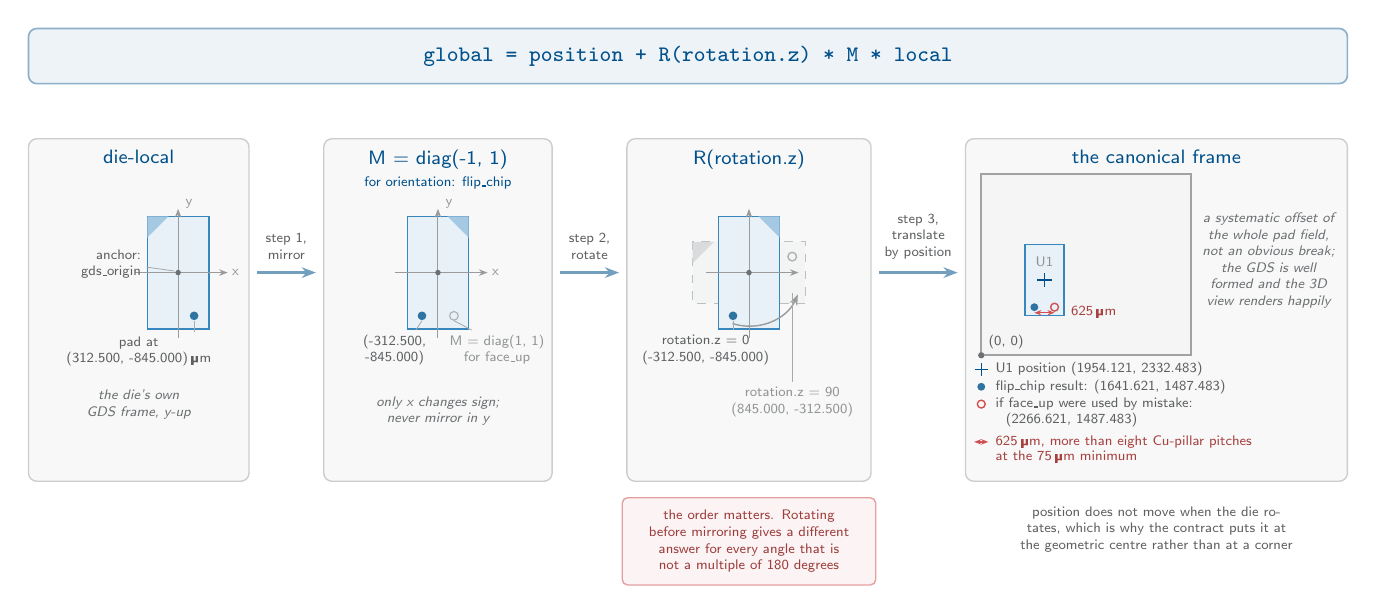
\begin{tikzpicture}[
    >=Stealth,
    adkpanel/.style={
        rectangle, rounded corners=3pt,
        draw=IHPaccent!35, fill=IHPaccent!5, line width=0.5pt
    },
    adkbanner/.style={
        rectangle, rounded corners=3pt,
        draw=IHPfg!45, fill=IHPfg!7, line width=0.6pt
    },
    adkptitle/.style={
        font=\sffamily\scriptsize, text=IHPfg, align=center, inner sep=1pt
    },
    adkcoord/.style={
        font=\sffamily\tiny, text=IHPaccent!85!black, align=center, inner sep=1pt
    },
    adkghostlbl/.style={
        font=\sffamily\tiny, text=IHPaccent!75, align=center, inner sep=1pt
    },
    adknote/.style={
        font=\sffamily\tiny\itshape, text=IHPaccent, align=center, inner sep=1pt
    },
    adkerrlbl/.style={
        font=\sffamily\tiny, text=cErr!80!black, align=left, inner sep=1pt
    },
    adkaxis/.style={-{Stealth[length=1.1mm]}, line width=0.35pt, color=IHPaccent!70},
    adkleader/.style={line width=0.3pt, color=IHPaccent!60},
    adkarrow/.style={-{Stealth[length=1.8mm]}, line width=0.8pt, color=IHPfg!55},
    adkrot/.style={-{Stealth[length=1.4mm]}, line width=0.5pt, color=IHPaccent!70},
    adkdim/.style={
        {Stealth[length=0.9mm]}-{Stealth[length=0.9mm]},
        line width=0.5pt, color=cErr
    },
    adkdie/.style={fill=cDieA!12, draw=cDieA, line width=0.5pt},
    adkghost/.style={fill=IHPaccent!8, draw=IHPaccent!45, line width=0.4pt, dashed},
    adkwarn/.style={
        rectangle, rounded corners=2pt,
        draw=cErr!55, fill=cErr!6, line width=0.5pt,
        text width=29mm, align=center, inner sep=1.6mm,
        font=\sffamily\tiny, text=cErr!75!black
    }
]

% =====================================================================
% Formula banner
% =====================================================================
\draw[adkbanner] (0, 5.05) rectangle (16.75, 5.75);
\node[font=\ttfamily\footnotesize, text=IHPfg] at (8.375, 5.40)
    {global = position + R(rotation.z) * M * local};

% =====================================================================
% Panel boxes
% =====================================================================
\draw[adkpanel] (0.00, 0) rectangle (2.80, 4.35);
\draw[adkpanel] (3.75, 0) rectangle (6.65, 4.35);
\draw[adkpanel] (7.60, 0) rectangle (10.70, 4.35);
\draw[adkpanel] (11.90, 0) rectangle (16.75, 4.35);

% =====================================================================
% PANEL 1: die-local
% =====================================================================
\node[adkptitle, anchor=north] at (1.40, 4.25) {die-local};

% die body, GDS origin at (1.90, 2.65). The die outline is schematic: only the
% pad coordinate is a documented number, so no die extent is labelled.
\draw[adkdie] (1.51, 1.935) rectangle (2.29, 3.365);
\fill[cDieA!45] (1.51, 3.365) -- (1.78, 3.365) -- (1.51, 3.095) -- cycle;

% axes
\draw[adkaxis] (1.35, 2.65) -- (2.53, 2.65);
\draw[adkaxis] (1.90, 1.82) -- (1.90, 3.46);
\node[adkghostlbl] at (2.63, 2.65) {x};
\node[adkghostlbl] at (2.04, 3.52) {y};

% origin
\fill[IHPaccent] (1.90, 2.65) circle (0.035);
\node[adkcoord, anchor=east, align=right] at (1.47, 2.76)
    {anchor:\\gds\_origin};
\draw[adkleader] (1.50, 2.72) -- (1.85, 2.67);

% pad
\fill[cDieA!85!black] (2.103, 2.101) circle (0.055);
\draw[adkleader] (2.103, 2.04) -- (2.103, 1.90);
\node[adkcoord, anchor=north] at (1.40, 1.88)
    {pad at\\(312.500, -845.000)\,\textmu m};

\node[adknote, anchor=north] at (1.40, 1.20)
    {the die's own\\GDS frame, y-up};

% =====================================================================
% PANEL 2: mirror
% =====================================================================
\node[adkptitle, anchor=north] at (5.20, 4.25)
    {M = diag(-1, 1)\\{\tiny for orientation: flip\_chip}};

% die body mirrored, origin at (5.20, 2.65)
\draw[adkdie] (4.81, 1.935) rectangle (5.59, 3.365);
\fill[cDieA!45] (5.59, 3.365) -- (5.32, 3.365) -- (5.59, 3.095) -- cycle;

\draw[adkaxis] (4.65, 2.65) -- (5.83, 2.65);
\draw[adkaxis] (5.20, 1.82) -- (5.20, 3.46);
\node[adkghostlbl] at (5.93, 2.65) {x};
\node[adkghostlbl] at (5.34, 3.52) {y};

\fill[IHPaccent] (5.20, 2.65) circle (0.035);

% mirrored pad
\fill[cDieA!85!black] (4.997, 2.101) circle (0.055);
\draw[adkleader] (4.997, 2.04) -- (4.92, 1.92);
\node[adkcoord, anchor=north] at (4.65, 1.90)
    {(-312.500,\\-845.000)};

% ghost of the unmirrored pad
\draw[color=IHPaccent!55, line width=0.4pt] (5.403, 2.101) circle (0.055);
\draw[adkleader] (5.403, 2.04) -- (5.63, 1.92);
\node[adkghostlbl, anchor=north] at (5.95, 1.90)
    {M = diag(1, 1)\\for face\_up};

\node[adknote, anchor=north] at (5.20, 1.12)
    {only x changes sign;\\never mirror in y};

% =====================================================================
% PANEL 3: rotate
% =====================================================================
\node[adkptitle, anchor=north] at (9.15, 4.25) {R(rotation.z)};

% ghost die, rotated 90 degrees counter-clockwise about the origin
\begin{scope}[shift={(9.15, 2.65)}, rotate=90]
    \draw[adkghost] (-0.39, -0.715) rectangle (0.39, 0.715);
    \fill[IHPaccent!25] (0.39, 0.715) -- (0.12, 0.715) -- (0.39, 0.445) -- cycle;
    \draw[color=IHPaccent!55, line width=0.5pt] (0.203, -0.549) circle (0.055);
\end{scope}

% solid die at rotation.z = 0
\draw[adkdie] (8.76, 1.935) rectangle (9.54, 3.365);
\fill[cDieA!45] (9.54, 3.365) -- (9.27, 3.365) -- (9.54, 3.095) -- cycle;

\draw[adkaxis] (8.60, 2.65) -- (9.78, 2.65);
\draw[adkaxis] (9.15, 1.82) -- (9.15, 3.46);
\fill[IHPaccent] (9.15, 2.65) circle (0.035);

% rotation arc
\draw[adkrot] ([shift=(252:0.68)]9.15, 2.65)
    arc[start angle=252, end angle=336, radius=0.68];

% pads
\fill[cDieA!85!black] (8.947, 2.101) circle (0.055);
\draw[adkleader] (8.947, 2.04) -- (8.947, 1.92);
\node[adkcoord, anchor=north] at (8.60, 1.90)
    {rotation.z = 0\\(-312.500, -845.000)};

\draw[adkleader] (9.699, 2.39) -- (9.699, 1.26);
\node[adkghostlbl, anchor=north] at (9.70, 1.24)
    {rotation.z = 90\\(845.000, -312.500)};

% =====================================================================
% PANEL 4: the canonical frame
% =====================================================================
\begin{scope}[xshift=2.5mm]
\node[adkptitle, anchor=north] at (14.075, 4.25) {the canonical frame};

% interposer GDS bbox
\draw[fill=IHPaccent!7, draw=IHPaccent!65, line width=0.6pt]
    (11.85, 1.60) rectangle (14.516, 3.90);
\fill[IHPaccent] (11.85, 1.60) circle (0.04);
\node[adkcoord, anchor=south west] at (11.90, 1.64) {(0, 0)};

% die U1 at its placed location
\draw[adkdie] (12.4061, 2.1061) rectangle (12.8989, 3.0096);
\node[adkghostlbl, anchor=south] at (12.6525, 2.68) {U1};

% geometric centre
\draw[line width=0.5pt, color=IHPfg]
    (12.5625, 2.5578) -- (12.7425, 2.5578)
    (12.6525, 2.4678) -- (12.6525, 2.6478);

% pads
\fill[cDieA!85!black] (12.5242, 2.2108) circle (0.05);
\draw[color=cErr, line width=0.5pt] (12.7808, 2.2108) circle (0.05);
\draw[adkdim] (12.5242, 2.14) -- (12.7808, 2.14);
\node[adkerrlbl, anchor=west] at (12.95, 2.15) {625\,\textmu m};

% caption, in the free column to the right of the interposer
\node[adknote, anchor=north, text width=17mm] at (15.50, 3.45)
    {a systematic offset of the whole pad field, not an obvious break;
     the GDS is well formed and the 3D view renders happily};

% legend
\draw[line width=0.5pt, color=IHPfg]
    (11.77, 1.42) -- (11.93, 1.42) (11.85, 1.34) -- (11.85, 1.50);
\node[adkcoord, anchor=west] at (11.99, 1.42)
    {U1 position (1954.121, 2332.483)};

\fill[cDieA!85!black] (11.85, 1.20) circle (0.05);
\node[adkcoord, anchor=west] at (11.99, 1.20)
    {flip\_chip result: (1641.621, 1487.483)};

\draw[color=cErr, line width=0.5pt] (11.85, 0.98) circle (0.05);
\node[adkcoord, anchor=west] at (11.99, 0.98)
    {if face\_up were used by mistake:};
\node[adkcoord, anchor=west] at (12.12, 0.78)
    {(2266.621, 1487.483)};

\draw[adkdim] (11.76, 0.50) -- (11.94, 0.50);
\node[adkerrlbl, anchor=west] at (11.99, 0.50)
    {625\,\textmu m, more than eight Cu-pillar pitches};
\node[adkerrlbl, anchor=west] at (11.99, 0.31)
    {at the 75\,\textmu m minimum};
\end{scope}

% =====================================================================
% Step arrows between the panels
% =====================================================================
\draw[adkarrow] (2.90, 2.65) -- (3.65, 2.65);
\node[adkcoord, anchor=south] at (3.275, 2.78) {step 1,\\mirror};

\draw[adkarrow] (6.75, 2.65) -- (7.50, 2.65);
\node[adkcoord, anchor=south] at (7.125, 2.78) {step 2,\\rotate};

\draw[adkarrow] (10.80, 2.65) -- (11.80, 2.65);
\node[adkcoord, anchor=south] at (11.30, 2.78) {step 3,\\translate\\by position};

% =====================================================================
% Notes below the panels
% =====================================================================
\node[adkwarn, anchor=north] at (9.15, -0.20)
    {the order matters. Rotating before mirroring gives a different answer for
     every angle that is not a multiple of 180 degrees};

\node[font=\sffamily\tiny, text=IHPaccent!85!black, align=center,
      anchor=north, text width=46mm] at (14.325, -0.20)
    {position does not move when the die rotates, which is why the contract
     puts it at the geometric centre rather than at a corner};

\end{tikzpicture}
\end{document}
